
\lecture{Normal Approximation of the Binomial}{normal-approximation-to-binomial}
\part{Normal Approximation of the Binomial}

\title{Normal Approximation of the Binomial}
\subtitle{Making the Binomial Distribution Tractable}

\author{Kelly Black}
\institute{Clarkson University}
\date{22 February 2012}

\begin{frame}
  \titlepage
\end{frame}

\begin{frame}
  \frametitle{Outline}
  \tableofcontents[pausesection,hideallsubsections,part=1]
\end{frame}


\section{Clicker Quiz}


\begin{frame}
  \frametitle{Clicker Quiz}

  Determine the value of $a$ that satisfies
  \begin{eqnarray*}
    p(z \leq a) & = & 0.95.
  \end{eqnarray*}

  \vfill

  \begin{tabular}{l@{\hspace{3em}}l@{\hspace{3em}}l}
    A: .8289 & B: 1.565 & C: 1.645
  \end{tabular}

  \vfill
  \vfill
  \vfill


\end{frame}




\section{Normal Distribution}

\begin{frame}
  \frametitle{Example}

  A random variable, $X$, is normally distributed with mean 2.5 and a
  standard deviation of 3.6. Find $a$ so that
  \begin{eqnarray*}
    p(-2.0 \leq X \leq a) & = & 0.80.
  \end{eqnarray*}

\end{frame}

\section{Binomial Approximation}

\begin{frame}

  \begin{block}{Binomial Approximation}
    Suppose that $X$ is a random variable that follows a binomial
    distribution. It has $N$ repetitions, and the probability of a
    success is $p$. 

    \textbf{IF} $N\cdot p\geq 5$ \textbf{AND} $N\cdot (1-p) \geq 5$
    then $X$ can be approximated using a normal distribution:

    \begin{center}
      \begin{tabular}{ll}
        Mean: & $N\cdot p$, \\
        Std. Dev. & $\sqrt{N\cdot p \cdot (1-p)}$,
      \end{tabular}
    \end{center}

    and

    \begin{eqnarray*}
      p(X \leq a) & \approx &
       p\lp Z \leq \frac{a+0.5-N\cdot p}{\sqrt{N\cdot p \cdot (1-p)}}\rp.
    \end{eqnarray*}

  \end{block}

\end{frame}

\begin{frame}{Binomial Distribution}

  \only<1>{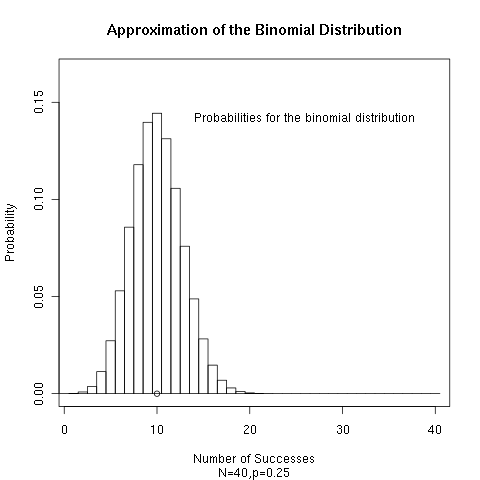
\includegraphics[width=6cm]{img/binomialN40}}
  \only<2>{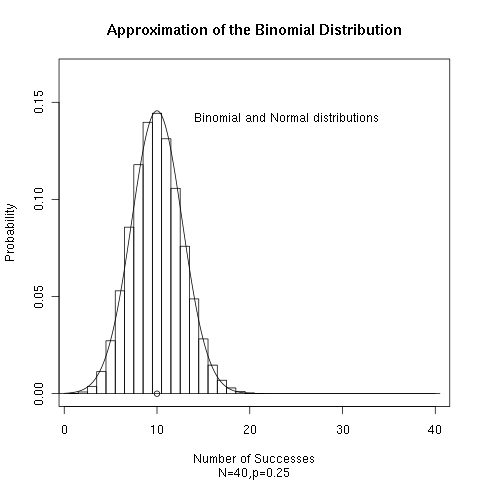
\includegraphics[width=6cm]{img/binomialApproximationN40}}
  
\end{frame}

\section{Examples}

\begin{frame}{Example}
  You want to take a poll of eighty employees. You will ask them if
  they like their benefits package. You suspect that 35\% of all
  employees do like their benefits. What is the probability that
  twenty-two or less will say they do?
\end{frame}


\begin{frame}{Example}
  You want to take a poll of eighty employees. You will ask them if
  they like their benefits package. You suspect that 35\% of all
  employees do like their benefits. Determine the cut-off where there
  is a twenty-five percent chance that fewer than the cut-off will say
  they do like their benefits.
\end{frame}


\begin{frame}{Clicker Quiz}
  Clarkson University claims that over eighty percent of all students
  take part in intramural sports. You choose three hundred students at
  random. What is the probability that more than two-hundred and fifty will say
  that they take part in intramural sports?

  \vfill

  \begin{tabular}{l@{\hspace{3em}}l@{\hspace{3em}}l}
    A: 0.0643  & B: 0.4679 & C: 0.9375
  \end{tabular}

  \vfill
  \vfill
  \vfill

\end{frame}



% LocalWords:  Clarkson pausesection hideallsubsections
